\section{Design of Recluse}
\label{sec:protocol} 
The overview of login flow is shown in Figure~\ref{fig:overview}, which contains RP identifier negotiation, dynamic registration and token obtaining. 
\begin{figure}
  \centering
  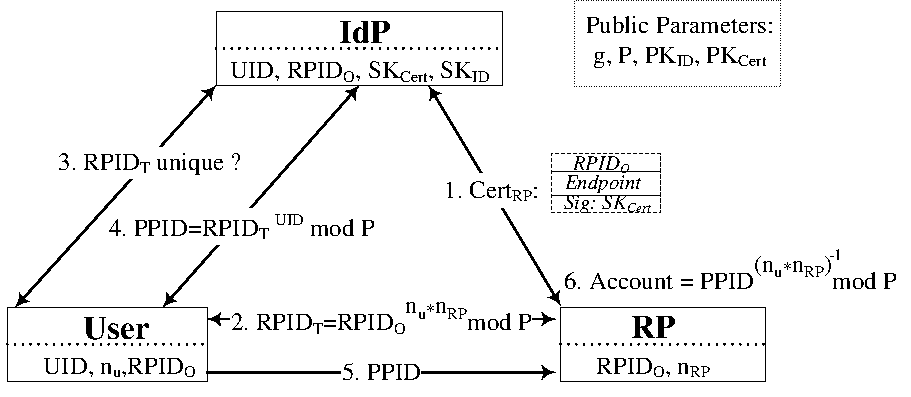
\includegraphics[width=\linewidth]{fig/Overview.pdf}
  \caption{Overview of System}
  \label{fig:overview}
\end{figure}
The of each phase in login flow is shown as follows:
\begin{itemize}
\item[1.] RP identifier Negotiation: For each SSO procedure, user is going to start negotiation with user. RP identifier is a random number which does not represent any RP, generated by rp-id-generating algorithm. However, the identifier is bound with specific authentication which is able to be confirmed by user and RP.
\item[2.] Dynamic Registration: To make the RP identifier generated by negotiation is valid in IdP, user is to register this identifier with IdP through the dynamic registration API provided by IdP. IdP is going to check whether the identifier is unique and require RP to restart identifier negotiation if the identifier has be used by another RP.
\item[3.] Authentication: After dynamic registration, RP builds the authentication request and redirects it to IdP through user agent. After receiving the request, IdP firstly authenticates user and then issues identity proof for RP, which contains the user id generated through the user-id-generating algorithm. Then IdP redirects the identity to RP through user agent, and RP identify the user through identity proof. 
\end{itemize}

\subsection{Prior Registration}
The prior registration between RP and IdP is shown as Figure~\ref{fig:registration}. 
\begin{figure}
  \centering
  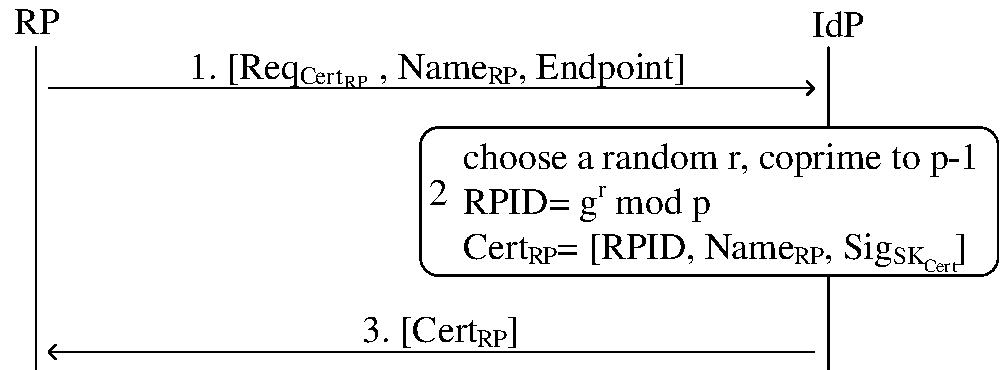
\includegraphics[width=\linewidth]{fig/registration.pdf}
  \caption{Prior Registration}
  \label{fig:registration}
\end{figure}
The registration process is as follows:
\begin{itemize}
\item[1.] Uploading Attributes: Firstly, IdP generates its prime $P$, the primitive root $g$ of $P$, the key pair \verb+pk+ and \verb+sk+. Then RP uploads it attributes, such as its name, endpoint, identity proof (e.g., business license) and so on.
\item[2.] Issuing RP Certification: IdP verifies the identity of RP and generates the RP certification including \verb+basic\_rp\_id+, \verb+rp\_name+, \verb+redirect\_uri+ and \verb+IdP\_origin+. IdP returns the RP certification, $P$, the key pair to RP.
\end{itemize}
The prior registration required for IdP to verify the basic attributes of RP, such as name, endpoints for identity proof, so that Idp is able to provide the RP certification to RP which includes the unique identifier for each RP and its attributes. With the RP certification, user agent has the ability to verify the RP's endpoint for identity proof and notify user with RP's identity. Additionally, the parameters, prime $P$ (used for user id generating) with its generator $g$, public key of IdP \verb+pk+ is provided in registration as well. 
Same as RP, user need to register with IdP and IdP generates unique user id for each user.


\subsection{Rp-id-generating and User-id-generating algorithm}
The rp-id-generating and user-id-generating algorithm are created based on Discrete Logarithm problem\cite{shiu2007cryptography:}.
IdP carefully chooses a big prime $P$\footnotetext[1]{$P$ is generated as $P=q\cdot 2+1$, while $q$ is prime as well.} and its primitive root \verb+g+ as generator for system. When the RP registers with IdP, IdP provides a unique primitive root as the RP's root identifier (called \verb+basic_rp_id+). 

The generation of \verb+rp_id+ and \verb+user_id+ is shown as Figure~\ref{fig:generating}, as well as the trapdoor for RP to derive \verb+user_rp_id+ is as shown.

\begin{figure*}
  \centering
  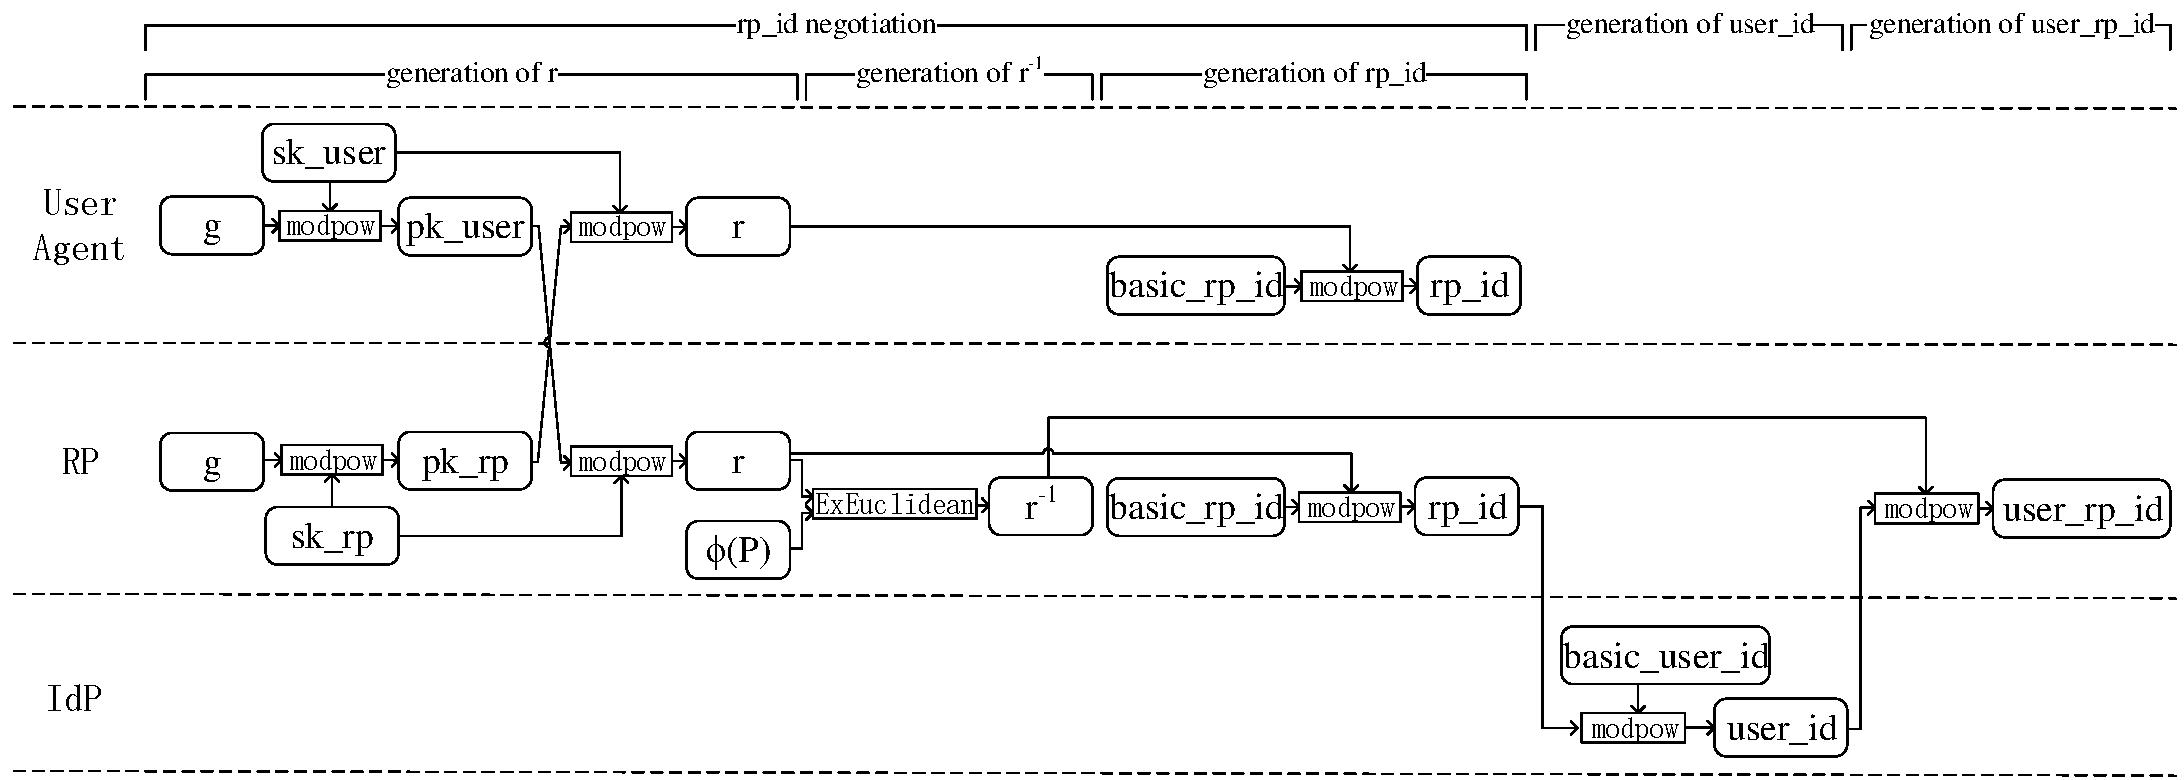
\includegraphics[width=\linewidth]{fig/generating3.pdf}
  \caption{Generation of rp\_id and user\_id}
  \label{fig:generating}
\end{figure*}

For each login process, the user and RP negotiate the temporary RP identifier bound with specific authentication.
While starting a login procedure, there is Diffie-Hellman key Exchange\cite{DiffieH76} between RP and user, through which the random $r$ is generated. However, to make sure that there is $r^{-1}$, that $r\cdot r^{-1}=1 mod \phi(P)$, $r$ should be the relative prime of $\phi(P)$, so that if $r$ is even $r$ should be added by one. Although there is little possibility that $r$ is the multiple of $p$ or $q$, it is not considered in the illustration. However, the re-negotiation is required in the practical system if $r$ is the multiple of $p$ or $q$. The RP identifier is generated as: 
$$rp\_id=basic\_rp\_id^r mod P\eqno(1)$$
such that $rp_id$ is another primitive element module \emph{p}. And $r^{-1}$ is generated through Extended Euclidean algorithm.

IdP labels each user at IdP with the unique identifier called $baisc\_user\_id$. To generate the specific user identifier for each $rp\_id$, the algorithm is 
$$user\_id=rp\_id^{basic\_user\_id} mod P\eqno(2)$$
so
$$user\_id=basic\_rp\_id^{r\cdot basic\_user\_id}modP\eqno(3)$$
While receiving $user\_id$ from IdP, RP can derive the constant user identifier from if
$$user\_rp\_id=user\_id^{r^{-1}} mod P\eqno(4)$$
so
$$user\_rp\_id=basic\_rp\_id^{(1 mod \phi(P))\cdot basic\_user\_id} mod P\eqno(5)$$
so
$$user\_rp\_id=basic\_rp\_id^{basic\_user\_id} mod P\eqno(6)$$
For single user in a RP, $user\_rp\_id$ is unchanged. However, $user\_rp\_id$s are distinct in each RP because $basic\_rp\_id$s are different in each RP.



\subsection{Login Flow}
The login flow is shown as Figure~\ref{fig:process}.
\begin{figure*}
  \centering
  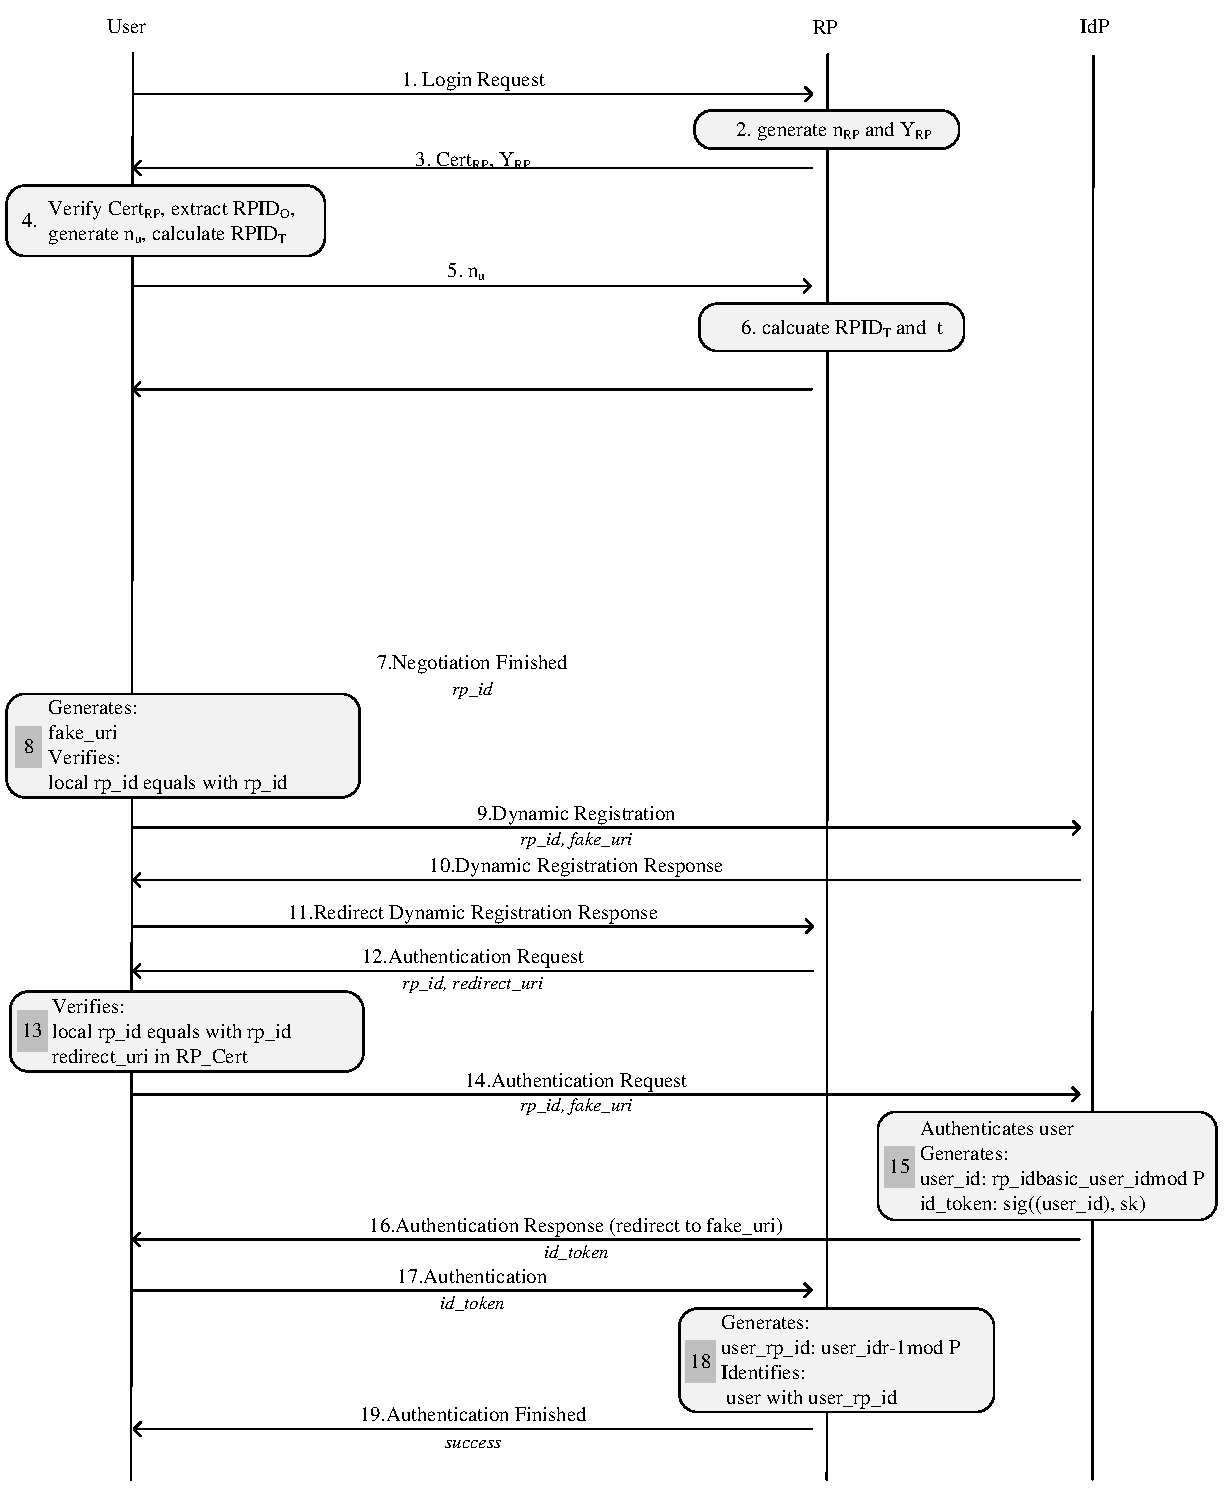
\includegraphics[width=\linewidth]{fig/process.pdf}
  \caption{Login Flow}
  \label{fig:process}
\end{figure*}

%抵抗phishing攻击:一定需要正确的RP参与,攻击者作为中间人
%1.使用IdP提供应用basic_rp_id与url的绑定,user agent保存映射
%缺点:占用空间,user agent需要缓存整个映射
%2.RP与用户通过加密的通道传输redirect_uri

%如果由RP选择basic_rp_id,那么多个rp之间的basic_rp_id有幂次关系,那么就可以关联用户

\subsubsection{RP Identifier Negotiation}
RP identifier negotiation starts form step 1 to step 4. The user accesses the service provided by RP in his/her browser. To log in this RP, user needs to click the login button offered by Recluse. 
Firstly, the user agent sends the \verb+Start Negotiation+ request to RP, so that RP generates the random $sk\_rp$ and $pk\_rp=g^{sk\_rp}modP$ as the private key and public key for DH Key exchanging. 
Secondly, RP builds the \verb+Negotiation Response+ with newly generated $pk\_rp$ as well as the \verb+RP_Cert+ issued by IdP. User agent similarly generates random $sk\_user$ and $pk\_user$, and $r=pk\_rp^{sk\_user}modP$. However, to make sure that $r$ is the relative prime of $\phi(P)$, it is required that $r$ should be odd and the greatest common divisor of $r$ and $\phi(P)$ is 1. 
Then user agent continues the \verb+Negotiation+ sending $pk\_user$ and $r$ to RP. RP generates the local $r$ in the same way as user agent and compares the local $r$ and user agent generated $r$. If $r$s are equal, RP generates $rp\_id=basic\_rp\_id^rmodP$, as well as $r^{-1}$ through Extend Euclidean algorithm, which meets $r\cdot r^{-1}=1mod\phi(P)$.
Finally RP transmits the $rp\_id$ to user agent. 
\subsubsection{Dynamic Registration}
Dynamic registration is from step 5 to step 7. While user agent receives teh $rp\_id$ from RP, it is required the $rp\_id$ from RP should be equal with it generated by user agent. Then user agent generates the \verb+fake\_uri+ which contains the random string and keeps it for further identity proof transmission. User agent sends the \verb+Dynamic Registration+ request to IdP with newly generated $rp\_id$ and \verb+fake_uri+ and redirects the \verb+Dynamic Registration Response+ to RP.
\subsubsection{Authentication}
Authentication is from step 8 to step 12. After dynamic registration,  RP builds the \verb+Authentication Request+ including $rp\_id$ as well as the \verb+redirect_uri+ representing the endpoint, and redirects it to IdP through user agent. User agent tampers the authentication request, compares $rp\_id$ with the local one, verifies the validation of the \verb+redirect_uri+ and replaces it with the fake one. Then user agent transmits the \verb+Authentication Request+ to IdP. After receiving the request, IdP firstly authenticates user and then generates $user\_id=rp\_id^{basic\_user\_id}modP$. The identity proof signed with IdP's private key including the $user\_id$ is redirected to the \verb+fake_uri+ through user agent, who intercepts the transmission and transmit it to the endpoint \verb+redirect_uri+ in authentication request. Finally, RP derives the constant $user\_rp\_id$ from $user\_id$. If the $user\_rp\_id$ has already been registered, RP send \verb+Authentication Finished+ with the message \verb+success+ to user agent.

%描述user_id, rp_id and user_rp_id的生成

